{\documentclass[12pt,a4paper, spanish]{report}
\usepackage[spanish]{babel}
\usepackage[latin1]{inputenc}  % Ambos para solucin de asuntos de idioma
\usepackage[T1]{fontenc}
\usepackage{tocbibind}  % Bibliografa en el indice
\usepackage{titlesec}  % Posibilidad de editar los formatos de chapter y section
%\usepackage{times}  % Fuente de letras
\usepackage{amsmath,amssymb,mathrsfs,mathptmx}  % Matemticas varias
\usepackage{hyperref} % Para escribir URLs

\usepackage[]{algorithm2e}
\usepackage{listings}
% \usepackage{keyval,fancyvrb,xcolor,float,ifthen,calc,ifplatform}
% \usepackage{minted}



% --- Arreglos varios para la inclusion de imgenes
%\usepackage[pdftex]{graphicx}
%\usepackage[dvips]{graphicx}
\usepackage{graphicx}
\usepackage{epstopdf}
% \usepackage{epsfig}
\usepackage{float}
\usepackage{subfigure}
% \usepackage{subfig}
\usepackage{wrapfig}
\usepackage[usenames,dvipsnames]{color}
\DeclareGraphicsExtensions{.png,.jpg,.pdf,.mps,.gif,.bmp, .eps}


\usepackage{multirow}
\usepackage{multicol}
\usepackage{tabulary}
\usepackage[table]{xcolor}
\usepackage{color}
\usepackage{listings}
%\usepackage{subfloat}
\usepackage{tikz}

\setcounter{secnumdepth}{3}
\setcounter{tocdepth}{3}


% --- Para las dimensiones de los mrgenes etc
\frenchspacing \addtolength{\hoffset}{-1.5cm}
\addtolength{\textwidth}{3cm} \addtolength{\voffset}{-2.5cm}
\addtolength{\textheight}{4cm}
% --- Para el encabezado
\usepackage{fancyhdr}
\fancyhead[R]{2012}\fancyhead[L]{enCuadro} \fancyfoot[C]{\thepage}
\pagestyle{fancy}

% --- Formato de la etiqueta Chapter
%\newcommand{\bigrule}{\titlerule[0.5mm]}
%\titleformat{\chapter}[display]{\bfseries\Huge}
%{\Large\chaptertitlename\ \Large\thechapter}
%{0mm} {\filleft} [\vspace{0.5mm} \bigrule]

\titleformat{\chapter}[display]
{\normalfont\Large\filcenter}
{\titlerule[1pt]%
\vspace{1pt}%
\titlerule
\vspace{1pc}%
\LARGE\MakeUppercase{\chaptertitlename} \thechapter}
{1pc}
{\titlerule
\vspace{1pc}%
\Huge}

%-------------------------

\begin{document}
% Esto es para que se muestren todas las referencias aunque no se citen:
\nocite{*}

\renewcommand{\tablename}{Tabla}
\renewcommand{\theenumi}{\Roman{enumi}}
\renewcommand{\labelenumi}{[\textbf{\theenumi}]}
\renewcommand{\thefootnote}{\arabic{footnote}}
% --- Modificacin de entornos enumerate
\renewcommand{\theenumi}{\roman{enumi}}
\renewcommand{\labelenumi}{\theenumi)}
% --- Modificacin de entornos enumerate

% --- Para hacer highlights
\newcommand{\highlAmarillo}[1]{\colorbox{yellow}{#1}}
\newcommand{\highlVerde}[1]{\colorbox{green}{#1}}
\newcommand{\highlRojo}[1]{\colorbox{red}{#1}}



v0.3
\chapter{Benchmark}
\label{chap: benchmark}
Durante el desarrollo del proyecto se hizo presente la necesidad de contar con herramientas de medida del desempe�o objetivas para la validaci�n de los algoritmos que se utilizaron y desarrollaron. En particular se desea evaluar los algoritmos asociados a la detecci�n y estimaci�n de pose. Estos son LSD, filtrado de segmentos, determinaci�n de correspondencias y Posit Coplanar. 

El enfoque elegido para la validaci�n de dichos algoritmos consiste en la generaci�n de una ``verdad de piso'' o \emph{ground truth} de forma de poder comparar la detecci�n y resultados obtenidos con los valores reales o verdaderos de los mismos. Este proceso es lo que se denomina en ese proyecto como \emph{Benchmark} o Comparativa. De esta forma se pueden generar un n�mero suficiente de datos de salida de forma de obtener algunas estad�sticas de inter�s para la evaluaci�n de los algoritmos.

\section{Generaci�n de im�genes sint�ticas: Blender}
La generaci�n de im�genes sint�ticas consiste en producir una imagen 2D en base a una modelo 3D de una escena y una pose de la c�mara respecto a esa escena o viceversa. Este proceso se denomina \emph{Rendering} y el mismo trata en el Cap�tulo \ref{chap: render} para la herramienta para dispositivos m�viles \emph{ISGL3D}. 

Para realizar el Benchmark se desarroll� un entorno de generaci�n de im�genes sint�ticas que utiliza herramientas gratuitas y de c�digo abierto que permiten capacidades de \emph{scripting} y ejecuci�n en forma ``batch'' de forma de serializar la producci�n de renders en un proceso autom�tico. En el proceso de estos renders fue realizada mediante el uso del software Blender.

Blender es un \emph{suite} de creaci�n de contenidos gratiuito y de c�digo abierto. Esta disponible para los principales sistemas operativos, Windows, Mac, Linux; bajo la Licencia P�blica General GNU\cite{blender}. Algunas de sus prestaciones son modelado, \emph{shading}, animaci�n, renderizado, e iteracci�n 3D. Tambi�n presenta herramientas de \emph{scripting} mediante el uso del lenguaje \emph{Python} las cuales se explicar�n mas adelante.

\subsection{Modelo 3D y escena}
Para lograr hacer un render es necesario contar con una escena 3D y en particular con un modelo 3D del objeto de inter�s. Para realizar las tareas de detecci�n se utiliza un marcador plano que se describe en el Cap�tulo \emph{ch:marcador}. 

Se manejaron algunas alternativas para la generaci�n del modelo 3D del marcador entre las cuales se encuentran, VTK, Paraview, Autodesk 3ds Max y el mismo programa utilizado por este proyecto para rendering en una PC, Blender. Finalmente debido a la simplicidad del marcador, y principalmente a que es un marcador plano, se utiliz� un dibujo vectorial del marcador (formato svg) generado en Inkscape. Este dibujo vectorial puede ser importado a Blender y con el generar un modelo 3D que ser� un actor en la escena. Dentro de la interfaz de Blender se ajust� un factor de escala para que las medidas reales del marcador se correspondan con las unidades de Blender. En la Figura \ref{fig:blender_usrprsp} se muestra la vista de \emph{Perspectiva de usuario} en donde se reflejan algunos de los cambios que se realizan sobre la escena.
\begin{figure}[h!]
  \centering
    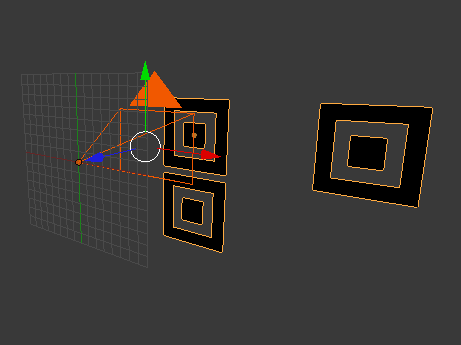
\includegraphics[scale=0.5]{figs_benchmark/blender/blender_usrprsp.png}
  \caption{Vista de perspectiva de usuario para el modelo 3D del marcador y la c�mara en la escena.}
  \label{fig:blender_usrprsp}
\end{figure}
Se busca construir una escena m�nima y controlada en la cual solo act�a el marcador. Con este fin es que se decide por una escena que contenga �nicamente el marcador y una c�mara. No se a�aden luces ya que el efecto de estas en el marcador para alguna pose puede resultar en artefactos de iluminaci�n indeseados. La no inclusi�n de luces en las imagen esta ligada a que el modelo 3D del marcador es en realidad hueco en las zonas blancas y negro en las zonas negras por lo tanto el negro permanece negro y la parte hueca asume el color del fondo. En otro caso se podr�a utilizar alg�n tipo de iluminaci�n de ambiente que sea pareja en todas las direcciones y lograr un efecto similar.\\

La escena conteniendo el modelo 3D del marcador se resume en el archivo \texttt{Marker.blend}.

\subsection{Ajuste de escena y par�metros}
El software Blender permite el ajuste de la escena y los par�metros y caracter�sticas asociados al render, la c�mara y el objeto mediante su interfaz gr�fica. Estos tienen como resultado final la imagen renderizada. Los par�metros y ajustes que fueron realizados y resultan ser los m�s relevantes para la reproducci�n del proceso de renderizado del marcador se explican a continuaci�n.

\begin{itemize}
 \item 
\textbf{Mundo y fondo}: Los ajustes realizados al mundo y fondo se explicaron en cierta medida anteriormente. Al no utilizar iluminaci�n en la escena es importante definir el color del fondo ya que los huecos del modelo 3D asumir�n ese color. Los ajustes realizados se muestran en la Figura \ref{fig:blender_props}(a) y consisten principalmente en definir el fondo de color blanco.

 \item 
\textbf{Parametros de Render}: Los principales par�metros ajustables en cuanto a las propiedades de render son el tama�o de imagen y el porcentaje de escala sobre el tama�o de imagen el cual por defecto en proyectos nuevos se ubica en $50\%$ y en este caso interesa que sea $100\%$. Estos ajustes se pueden ver en la Figura \ref{fig:blender_props}(b).

 \item 
\textbf{Par�metros de C�mara}: Sobre las propiedades ajustables de la c�mara se encuentra un par�metro de inter�s como es el campo visual, \emph{field of view}, o $fov$. Adicionalmente el \emph{Shift} representa el corrimiento del centro de imagen de la misma y tambi�n se puede ajustar en \emph{near} y el \emph{far}. Los ajustes realizados se pueden ver en la Figura \ref{fig:blender_props}(c).

 \item 
\textbf{Par�metros de Objeto}: Las propiedades ajustables de mayor inter�s sobre el objeto se refieren a su pose. La locaci�n y rotaci�n del objeto pueden ser asociadas a la pose del objeto respecto a la c�mara si se asume una interacci�n del tipo c�mara fija, objeto movil. Se aclara aqu� que un ajuste id�ntico se puede realizar sobre el objeto c�mara. La c�mara se fija para todos los casos en el origen de coordenadas de Blender con orientaci�n nula en las tres direcci�nes. Esto resulta en una c�mara que mira en el eje $z$. Volviendo a los ajustes del objeto marcador, se presentan los ajustes de escala ya mencionados en el ajuste de unidades del modelo 3D y tambi�n un factor de importancia como es el orden y tipo de rotaci�n \emph{XYZ Euler}. Todos los ajustes aqu� descritos para el objeto marcadores se pueden ver en la Figura \ref{fig:blender_props}(d).
\end{itemize}
Vale la pena observar que los ajustes de Render y C�mara constituyen una forma de establecer los \textbf{par�metros intr�nsecos} de la c�mara. Mientras que los ajustes de Objeto para la C�mara y el Marcador representan la \textbf{pose del objeto} en el modelo de vinculaci�n adoptado. Se aclara que los \textbf{par�metros extr�nsecos} de la c�mara respecto a las coordenadas de Blender es nula en rotaci�n y traslaci�n.
\begin{figure}[h!]
  \centering
  \subfigure[Ajustes de mundo y fondo]{
    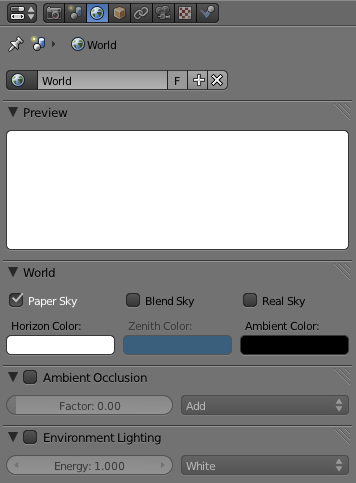
\includegraphics[scale=0.5]{figs_benchmark/blender/blender_wrldprops.png}}
    \label{fig:blender_props_a}
  \subfigure[Ajustes de render]{
    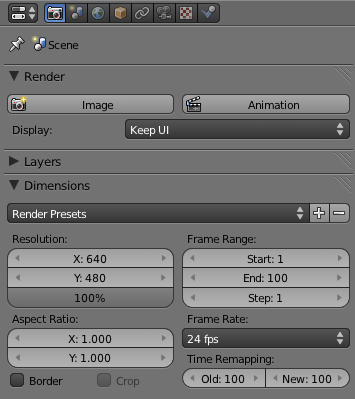
\includegraphics[scale=0.5]{figs_benchmark/blender/blender_rndrprops.png}}
    \label{fig:blender_props_b}
  \subfigure[Ajustes de c�mara]{
    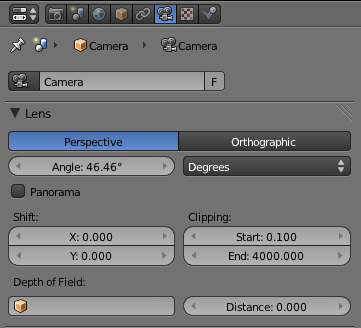
\includegraphics[scale=0.5]{figs_benchmark/blender/blender_cameraprops.png}}
    \label{fig:blender_props_c}
  \subfigure[Pose del objeto]{
    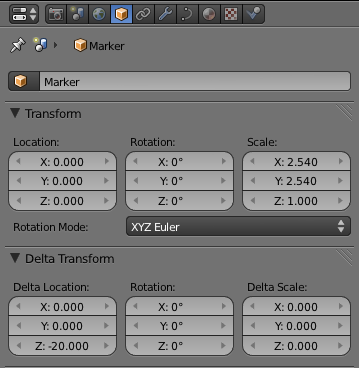
\includegraphics[scale=0.5]{figs_benchmark/blender/blender_objprops.png}}
    \label{fig:blender_props_d}
  \caption{Ajustes en la escena en Blender para realizar el render.}
  \label{fig:blender_props}
\end{figure}

\subsection{Python scripting}
Python es un lenguaje de programaci�n interpretado, interactivo y orientado a objetos. Incorpora m�dulos, excepciones, tipeo din�mico, tipos de datos de muy alto nivel y clases. Python logra combinar not�blemente poder con claridad en la sintaxis \cite{blender_python}. La mayor�a de las �reas de Blender pueden ser programadas mediante \emph{scripts}, incluyendo Animaci�n, Renderizado, Importaci�n y Exportaci�n, Creaci�n de objetos y tareas repetitivas. Para la interacci�n con Blender se hace uso de una API ``ajustada a medida''.

La API de Blender para Python se encuentra empaquetada en el m�dulo \texttt{bpy}. Mediante este m�dulo se puede acceder a los objetos y sus propiedades de la escena. De esta forma se puede de forma program�tica ajustar las propiedades y par�metros explicados anteriormente. De esta forma mediante la interprete de comandos de Blender se puede prescindir de la interfaz gr�fica de Blender. En la Figura \ref{blender_pyconsole} se muestra un \emph{screenshot} de la consola interactiva de Python en Blender.
\begin{figure}[h!]
  \centering
    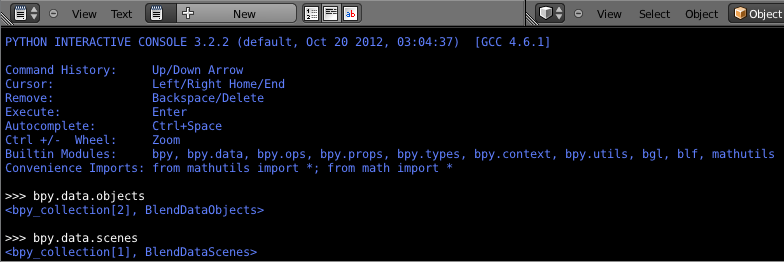
\includegraphics[scale=0.5]{figs_benchmark/blender/blender_pyconsole.png}
  \caption{Consola interactiva de Python incrustada en Blender.}
  \label{fig:blender_pyconsole}
\end{figure}

\begin{itemize}
 \item Obtener referencias a la escena y el marcador.
\begin{verbatim}
>>> scene = bpy.data.scenes["Scene"]
>>> marker = bpy.data.objects["Marker"]
\end{verbatim}
 
 \item Seleccionar modo de rotaci�n y ubicar y orientar c�mara como se desea.
\begin{verbatim}
>>> scene.camera.rotation_mode = 'XYZ'
>>> scene.camera.rotation_euler = [0,0,0]
>>> scene.camera.location = [0,0,0]
\end{verbatim}

 \item Asignaci�n de valores asociados a \textbf{par�metros intr�nsecos} de la c�mara.
\begin{verbatim}
>>> scene.render.resolution_x = width
>>> scene.render.resolution_y = height
>>> scene.camera.data.angle = fov*(pi/180.0)
\end{verbatim}

 \item Asignaci�n de valores asociados a la \textbf{pose} del marcador.
\begin{verbatim}
>>> marker.rotation_mode = 'XYZ'
>>> marker.rotation_euler = [rx,ry,rz]
>>> marker.location = [tx,ty,tz]
\end{verbatim}

 \item Asignaci�n de nombre de imagen renderizada y ejecuci�n de renderizado para guardar la imagen.
\begin{verbatim}
>>> bpy.data.scenes["Scene"].render.filepath = str(fname)
>>> bpy.ops.render.render( write_still=True ) 
\end{verbatim}
\end{itemize}

\subsection{Ejecuci�n de consola de comandos}

\bibliographystyle{unsrt}   
\bibliography{encuadro}  
\end{document}